\documentclass[12pt]{article}
\usepackage[margin=1in]{geometry}
\usepackage{amsmath,amssymb}
\usepackage{booktabs}
\usepackage{array}
\usepackage{graphicx}
\usepackage{float}
\usepackage{hyperref}
\hypersetup{
    colorlinks=true,
    linkcolor=blue,
    citecolor=blue,
    urlcolor=blue
}

\begin{document}

\title{\textbf{Homework 2}\\[0.5ex] \large Advanced Solid State}
\author{Janessa Slone \and Nathan Smith}
\date{}
\maketitle

\section{Overview}

In this assignment, we investigate the electronic band structure of two-dimensional crystalline systems using the tight-binding approximation in a non-orthogonal orbital basis. We formulate and solve the generalized eigenvalue secular equation for two distinct systems:
\begin{enumerate}
    \item \textbf{Part 1: Two-Orbital Square Lattice}: A square Bravais lattice containing two localized atomic orbitals ($\phi_1$ and $\phi_2$) per lattice site, characterized by on-site reference energies $\epsilon_1 = 0$ and $\epsilon_2 = 0.8\,t_0$. Hopping integrals $t_{nm}(R)$ and spatial overlap integrals $\eta_{nm}(R)$ decay exponentially with interatomic distance $R$, parameterized by a characteristic decay length $d_0$.
    \item \textbf{Part 2: Crystal B (Centered Rectangular Lattice)}: Inspired by the non-cubic symmetry of Crystal B from Homework~1, we model an anisotropic 2D centered rectangular lattice containing a two-site conventional basis with three total orbital states ($3\times 3$ secular problem). We examine intra-sublattice and inter-sublattice couplings along the high-symmetry path of the rectangular Brillouin zone.
\end{enumerate}

For both systems, electronic dispersions are computed along high-symmetry Brillouin zone contours across multiple lattice parameters ($a = 5\,d_0$, $7\,d_0$, and $9\,d_0$). We systematically evaluate three levels of physical approximation:
\begin{itemize}
    \item \textbf{Full Model (NN + NNN with Overlap)}: Nearest-neighbor (NN) and next-nearest-neighbor (NNN) interactions including full spatial overlap matrices $\mathbf{S}(\mathbf{k}) = \boldsymbol{\eta}(\mathbf{k})$.
    \item \textbf{NN-Only with Overlap}: Restriction of hopping and overlap matrices to nearest-neighbor shells.
    \item \textbf{Zero-Overlap Approximation}: Neglect of all off-site overlap integrals ($\eta_{nm}(\mathbf{R}) = \delta_{nm}\delta_{\mathbf{R},\mathbf{0}}$), yielding an orthogonal basis ($\mathbf{S} = \mathbf{I}$).
\end{itemize}

Finally, we conduct a rigorous numerical stability analysis. We uncover the physical origin of the dramatic energy divergences observed at small lattice constants ($a = 5\,d_0$), identifying the exact geometric threshold at which constructive interference of overlap integrals causes the overlap matrix $\mathbf{S}(\mathbf{k})$ to lose positive-definiteness. We also address the mathematical subtlety of non-Hermiticity in the effective single-matrix formulation $\mathbf{M} = \bar{\boldsymbol{\epsilon}} + \bar{\mathbf{t}}\bar{\boldsymbol{\eta}}^{-1}$ and demonstrate how a physically symmetrized Hamiltonian restores Hermiticity and numerical stability.

\section{Theoretical Framework and Tight-Binding Formalism}

\subsection{Bloch Basis with Non-Orthogonal Orbitals}

Consider a crystal with lattice vectors $\mathbf{R}$ and basis atoms located at positions $\boldsymbol{\tau}_n$ within the unit cell. To each atomic orbital $\phi_n$ centered at $\mathbf{R} + \boldsymbol{\tau}_n$, we construct a Bloch wave packet satisfying translation symmetry:
\begin{equation}
    \Phi_{n\mathbf{k}}(\mathbf{r}) = \frac{1}{\sqrt{N}} \sum_{\mathbf{R}} e^{i\mathbf{k}\cdot(\mathbf{R} + \boldsymbol{\tau}_n)} \phi_n(\mathbf{r} - \mathbf{R} - \boldsymbol{\tau}_n),
    \label{eq:bloch_basis}
\end{equation}
where $N$ is the total number of unit cells. Because the localized atomic orbitals $\{\phi_n\}$ are not mutually orthogonal across different lattice sites, the overlap matrix elements in the Bloch basis are given by:
\begin{equation}
    S_{nm}(\mathbf{k}) = \langle \Phi_{n\mathbf{k}} | \Phi_{m\mathbf{k}} \rangle = \sum_{\mathbf{R}} e^{i\mathbf{k}\cdot(\mathbf{R} + \boldsymbol{\tau}_m - \boldsymbol{\tau}_n)} \eta_{nm}(\mathbf{R}),
    \label{eq:overlap_matrix}
\end{equation}
where the two-center spatial overlap integral is defined as:
\begin{equation}
    \eta_{nm}(\mathbf{R}) = \int \phi_n^*(\mathbf{r}) \phi_m(\mathbf{r} - \mathbf{R}) \, d^2r.
\end{equation}
By spatial normalization of the isolated atomic states, $\eta_{nm}(\mathbf{0}) = \delta_{nm}$ for orbitals centered on the same atomic site.

The crystal Hamiltonian $\hat{H} = \hat{T} + \sum_{\mathbf{R}, j} V_{\text{at}}(\mathbf{r} - \mathbf{R} - \boldsymbol{\tau}_j)$ evaluated in this basis yields matrix elements:
\begin{equation}
    H_{nm}(\mathbf{k}) = \langle \Phi_{n\mathbf{k}} | \hat{H} | \Phi_{m\mathbf{k}} \rangle = \sum_{\mathbf{R}} e^{i\mathbf{k}\cdot(\mathbf{R} + \boldsymbol{\tau}_m - \boldsymbol{\tau}_n)} \int \phi_n^*(\mathbf{r} - \boldsymbol{\tau}_n) \hat{H} \phi_m(\mathbf{r} - \mathbf{R} - \boldsymbol{\tau}_m) \, d^2r.
\end{equation}
Within the standard tight-binding approximation, the atomic Hamiltonian satisfies $\hat{H}_{\text{at}}^{(m)}\phi_m = \bar{\epsilon}_m \phi_m$. Approximating the potential as the atomic potential plus a crystal perturbation $\Delta V(\mathbf{r})$, the Hamiltonian matrix elements separate into on-site energies, overlap contributions, and hopping integrals:
\begin{equation}
    H_{nm}(\mathbf{k}) = \sum_{\mathbf{R}} e^{i\mathbf{k}\cdot(\mathbf{R} + \boldsymbol{\tau}_m - \boldsymbol{\tau}_n)} \left[ \bar{\epsilon}_m \eta_{nm}(\mathbf{R}) + t_{nm}(\mathbf{R}) \right],
    \label{eq:hamiltonian_elements}
\end{equation}
where the transfer (hopping) parameter is defined by:
\begin{equation}
    t_{nm}(\mathbf{R}) = \int \phi_n^*(\mathbf{r} - \boldsymbol{\tau}_n) \Delta V(\mathbf{r}) \phi_m(\mathbf{r} - \mathbf{R} - \boldsymbol{\tau}_m) \, d^2r.
\end{equation}
By convention, crystal field shifts at $\mathbf{R} = \mathbf{0}$ are absorbed into the on-site atomic energies $\bar{\epsilon}_m$, setting $t_{nm}(\mathbf{0}) = 0$.

\subsection{Secular Equation and Generalized Eigenvalue Problem}

The crystal Schrödinger equation $\hat{H}\Psi_{\mathbf{k}} = E(\mathbf{k})\Psi_{\mathbf{k}}$ expanded in the Bloch basis $\Psi_{\mathbf{k}}(\mathbf{r}) = \sum_m c_m(\mathbf{k}) \Phi_{m\mathbf{k}}(\mathbf{r})$ leads directly to the generalized secular equation:
\begin{equation}
    \sum_{m} \left[ H_{nm}(\mathbf{k}) - E(\mathbf{k}) S_{nm}(\mathbf{k}) \right] c_m(\mathbf{k}) = 0.
    \label{eq:secular}
\end{equation}
Nontrivial solutions require the vanishing of the secular determinant:
\begin{equation}
    \det \left[ \mathbf{H}(\mathbf{k}) - E(\mathbf{k}) \mathbf{S}(\mathbf{k}) \right] = 0.
    \label{eq:secular_det}
\end{equation}
In matrix notation, let $\bar{\boldsymbol{\epsilon}} = \operatorname{diag}(\bar{\epsilon}_1, \dots, \bar{\epsilon}_N)$, $\bar{\boldsymbol{\eta}}(\mathbf{k}) \equiv \mathbf{S}(\mathbf{k})$, and define the hopping matrix:
\begin{equation}
    \bar{\mathbf{t}}(\mathbf{k}) = \sum_{\mathbf{R} \neq \mathbf{0}} e^{i\mathbf{k}\cdot(\mathbf{R} + \boldsymbol{\tau}_m - \boldsymbol{\tau}_n)} \mathbf{t}(\mathbf{R}).
\end{equation}
Then the Hamiltonian matrix can be written as $\mathbf{H}(\mathbf{k}) = \bar{\boldsymbol{\epsilon}}\bar{\boldsymbol{\eta}}(\mathbf{k}) + \bar{\mathbf{t}}(\mathbf{k})$. Whenever the overlap matrix $\bar{\boldsymbol{\eta}}(\mathbf{k})$ is non-singular, multiplying Eq.~\eqref{eq:secular} from the right by $\bar{\boldsymbol{\eta}}^{-1}$ casts the problem into a standard eigenvalue equation for an effective dynamical matrix $\mathbf{M}(\mathbf{k})$:
\begin{equation}
    \mathbf{M}(\mathbf{k})\mathbf{c}(\mathbf{k}) = E(\mathbf{k})\mathbf{c}(\mathbf{k}), \qquad \mathbf{M}(\mathbf{k}) \equiv \bar{\boldsymbol{\epsilon}} + \bar{\mathbf{t}}(\mathbf{k})\bar{\boldsymbol{\eta}}(\mathbf{k})^{-1}.
    \label{eq:M_matrix}
\end{equation}
Alternatively, to preserve strict Hermiticity in the presence of non-commuting on-site and overlap matrices ($[\bar{\boldsymbol{\epsilon}}, \bar{\boldsymbol{\eta}}] \neq 0$), the physical Hamiltonian is symmetrized:
\begin{equation}
    \mathbf{H}_{\text{sym}}(\mathbf{k}) = \frac{1}{2}\left[ \bar{\boldsymbol{\epsilon}}\bar{\boldsymbol{\eta}}(\mathbf{k}) + \bar{\boldsymbol{\eta}}(\mathbf{k})\bar{\boldsymbol{\epsilon}} \right] + \bar{\mathbf{t}}(\mathbf{k}),
    \label{eq:H_sym}
\end{equation}
which satisfies $\mathbf{H}_{\text{sym}}^\dagger = \mathbf{H}_{\text{sym}}$ and can be solved using generalized Hermitian eigensolvers.

\subsection{Distance-Dependent Overlap and Hopping Integrals}

The distance dependence of the overlap and hopping matrices between atomic orbitals 1 and 2 is parameterized analytically in terms of a characteristic decay length $d_0$ and an energy scale $t_0$. For interatomic separation $R > 0$:
\begin{align}
    \eta_{11}(R) &= \left( 1 + \frac{R}{d_0} + \frac{R^2}{3 d_0^2} \right) \exp\left(-\frac{R}{d_0}\right), \label{eq:eta11} \\
    \eta_{12}(R) &= \frac{1}{2}\left( 1 + \frac{R}{d_0} + \frac{R^2}{64 d_0^2} \right) \exp\left(-\frac{R}{2 d_0}\right) - \frac{1}{2}\exp\left(-\frac{R}{d_0}\right), \label{eq:eta12} \\
    \eta_{22}(R) &= \left( 1 + \frac{R}{2 d_0} + \frac{R^2}{24 d_0^2} \right) \exp\left(-\frac{R}{2 d_0}\right), \label{eq:eta22}
\end{align}
and the corresponding transfer (hopping) parameters are:
\begin{align}
    t_{11}(R) &= -t_0 \left( 1 + \frac{2R}{d_0} \right) \exp\left(-\frac{R}{d_0}\right), \label{eq:t11} \\
    t_{12}(R) &= -t_0 \left( 1 + \frac{2R}{d_0} \right) \exp\left(-\frac{R}{d_0}\right) + t_0 \left( 1 + \frac{R}{16 d_0} \right) \exp\left(-\frac{R}{2 d_0}\right), \label{eq:t12} \\
    t_{22}(R) &= -t_0 \left( 1 + \frac{R}{2 d_0} - \frac{R^2}{24 d_0^2} \right) \exp\left(-\frac{R}{2 d_0}\right). \label{eq:t22}
\end{align}
At $R = 0$, the boundary conditions are $\eta_{nm}(0) = \delta_{nm}$ and $t_{nm}(0) = 0$. The reference atomic energies are $\epsilon_1 = 0$ and $\epsilon_2 = 0.8\,t_0$, giving:
\begin{equation}
    \bar{\boldsymbol{\epsilon}} = \begin{pmatrix} 0 & 0 \\ 0 & 0.8\,t_0 \end{pmatrix}.
\end{equation}

\section{Crystal A: Square Lattice}

The square lattice has no lattice basis, therefore the only relevant $\boldsymbol{\tau}$ is $\boldsymbol{\tau} = (0,0)$, and there are only 2 orbitals, therefore the eigenvalue problem as a function of $\mathbf{k}$ will be $2 \times 2$. Corresponding to the two orbitals on-site.

Therefore $\bar{\boldsymbol{\epsilon}}$ is given by:
\begin{equation}
    \bar{\boldsymbol{\epsilon}} = \begin{pmatrix}
        0 & 0 \\
        0 & 0.8t_{0}
    \end{pmatrix}.
\end{equation}

\subsection*{Nearest Neighbor Contributions}

For the square lattice, this is straightforward. We consider one orbital pair as an example, and the rest follows by the same logic. Note also that the on-site contribution gives $\delta_{nm}$.

Using the set of nearest neighbor vectors $\mathbf{R}_{j} = (\pm a, 0), (0, \pm a)$ with $R = a$, since $\eta_{nm}$ and $t_{nm}$ depend only on distance $R$:
\begin{align}
    \eta^{(0)}_{nm}(\mathbf{k}) &= \sum_{\mathbf{R}_{\text{NN}}} \eta_{nm}(\mathbf{R}_{j}) e^{i \mathbf{k} \cdot \mathbf{R}_{j}} = \eta_{nm}(a) \left[ e^{i k_{x}a} + e^{-i k_{x}a} + e^{i k_{y}a} + e^{-i k_{y}a} \right] \nonumber \\
    &= 2 \eta_{nm}(a) \left[\cos(k_{x}a) + \cos(k_{y}a)\right] = 2 \eta_{nm}(a) \epsilon_{0}(\mathbf{k}),
\end{align}
where $\epsilon_{0}(\mathbf{k}) = \cos(k_{x}a) + \cos(k_{y}a)$. This factor is the same across all orbital pairs, so in general we can write:
\begin{align}
    \eta^{(0)}_{nm}(\mathbf{k}) &= 2 \eta_{nm}(a) \epsilon_{0}(\mathbf{k}), \\
    t^{(0)}_{nm}(\mathbf{k}) &= 2 t_{nm}(a) \epsilon_{0}(\mathbf{k}).
\end{align}

\subsection*{Next-Nearest Neighbor Contributions}

A similar logic follows for the next-nearest neighbors at $\mathbf{R}_{j} = (\pm a, \pm a)$ with distance $R = \sqrt{2}a$:
\begin{align}
    \eta^{(1)}_{nm}(\mathbf{k}) &= \eta_{nm}(\sqrt{2}a) \left[e^{i a(k_{x} + k_{y})} + e^{i a(k_{x} - k_{y})} + e^{-i a(k_{x} - k_{y})} + e^{-i a(k_{x} + k_{y})}\right] \nonumber \\
    &= 2 \eta_{nm}(\sqrt{2}a)\left[\cos(a k_{x} + a k_{y}) + \cos(a k_{x} - a k_{y})\right] \nonumber \\
    &= 4 \eta_{nm}(\sqrt{2}a) \cos(k_{x}a) \cos(k_{y}a) = 2 \eta_{nm}(\sqrt{2}a) \epsilon_{1}(\mathbf{k}),
\end{align}
where $\epsilon_{1}(\mathbf{k}) = \cos(a(k_{x} + k_{y})) + \cos(a(k_{x} - k_{y})) = 2 \cos(k_{x}a) \cos(k_{y}a)$.

The exact same is true for $t_{nm}$, so including the on-site term $\delta_{nm}$ for the overlap, we can write the total contributions as:
\begin{align}
    \eta_{nm}(\mathbf{k}) &= \delta_{nm} + 2 \eta_{nm}(a) \epsilon_{0}(\mathbf{k}) + 2 \eta_{nm}(\sqrt{2}a) \epsilon_{1}(\mathbf{k}), \label{eq:sq_eta} \\
    t_{nm}(\mathbf{k}) &= 2 t_{nm}(a) \epsilon_{0}(\mathbf{k}) + 2 t_{nm}(\sqrt{2}a) \epsilon_{1}(\mathbf{k}). \label{eq:sq_t}
\end{align}

The high-symmetry path traversing the first Brillouin zone is $\Gamma(0, 0) \to X\left(\frac{\pi}{a}, 0\right) \to M\left(\frac{\pi}{a}, \frac{\pi}{a}\right) \to \Gamma(0, 0)$.

\subsection{Analytical Solution for the 2D Dispersion}

Because the system is $2\times 2$, the eigenvalues of $\mathbf{M}(\mathbf{k}) = \bar{\boldsymbol{\epsilon}} + \bar{\mathbf{t}}(\mathbf{k})\bar{\boldsymbol{\eta}}(\mathbf{k})^{-1}$ can be solved in closed algebraic form. Evaluating the matrix inverse:
\begin{equation}
    \bar{\boldsymbol{\eta}}(\mathbf{k})^{-1} = \frac{1}{\det \bar{\boldsymbol{\eta}}(\mathbf{k})} \begin{pmatrix} \bar{\eta}_{22}(\mathbf{k}) & -\bar{\eta}_{12}(\mathbf{k}) \\ -\bar{\eta}_{12}(\mathbf{k}) & \bar{\eta}_{11}(\mathbf{k}) \end{pmatrix},
\end{equation}
with $\det \bar{\boldsymbol{\eta}}(\mathbf{k}) = \bar{\eta}_{11}(\mathbf{k})\bar{\eta}_{22}(\mathbf{k}) - \bar{\eta}_{12}(\mathbf{k})^2$. Computing $\det(\mathbf{M}(\mathbf{k}) - E\mathbf{I}) = 0$ yields the characteristic equation:
\begin{equation}
    E^2 - \operatorname{Tr}(\mathbf{M}) E + \det(\mathbf{M}) = 0,
\end{equation}
whose roots are:
\begin{equation}
    E_{1,2}(\mathbf{k}) = \frac{\operatorname{Tr}(\mathbf{M}(\mathbf{k})) \mp \sqrt{\operatorname{Tr}(\mathbf{M}(\mathbf{k}))^2 - 4\det(\mathbf{M}(\mathbf{k}))}}{2}.
    \label{eq:analytical_roots}
\end{equation}
Expanding this explicitly in terms of the components of $\bar{\boldsymbol{\epsilon}}$, $\bar{\boldsymbol{\eta}}$, and $\bar{\mathbf{t}}$ yields:
\begin{equation}
    E_{1,2}(\mathbf{k}) = \frac{\epsilon_2 \det\bar{\boldsymbol{\eta}} + \bar{\eta}_{11}\bar{t}_{22} - 2\bar{\eta}_{12}\bar{t}_{12} + \bar{\eta}_{22}\bar{t}_{11} \mp \sqrt{\Delta(\mathbf{k})}}{2 \det\bar{\boldsymbol{\eta}}(\mathbf{k})},
    \label{eq:expanded_roots}
\end{equation}
where the discriminant $\Delta(\mathbf{k})$ is given by:
\begin{align}
    \Delta(\mathbf{k}) &= \left[ \epsilon_2 \det\bar{\boldsymbol{\eta}} + \bar{\eta}_{11}\bar{t}_{22} - 2\bar{\eta}_{12}\bar{t}_{12} + \bar{\eta}_{22}\bar{t}_{11} \right]^2 \nonumber \\
    &\quad - 4\det\bar{\boldsymbol{\eta}} \left[ \epsilon_2 (\bar{t}_{11}\bar{\eta}_{22} - \bar{t}_{12}\bar{\eta}_{12}) + \bar{t}_{11}\bar{t}_{22} - \bar{t}_{12}^2 \right].
\end{align}
This analytical result reproduces the exact symbolic expression derived in scratch calculations.

\subsection{Electronic Band Structures across Lattice Parameters}

Figure~\ref{fig:part1_bands} presents the calculated dispersion relations along $\Gamma \to X \to M \to \Gamma$ for $a = 5\,d_0$, $7\,d_0$, and $9\,d_0$ under the full NN + NNN model with spatial overlap.

\begin{figure}[H]
    \centering
    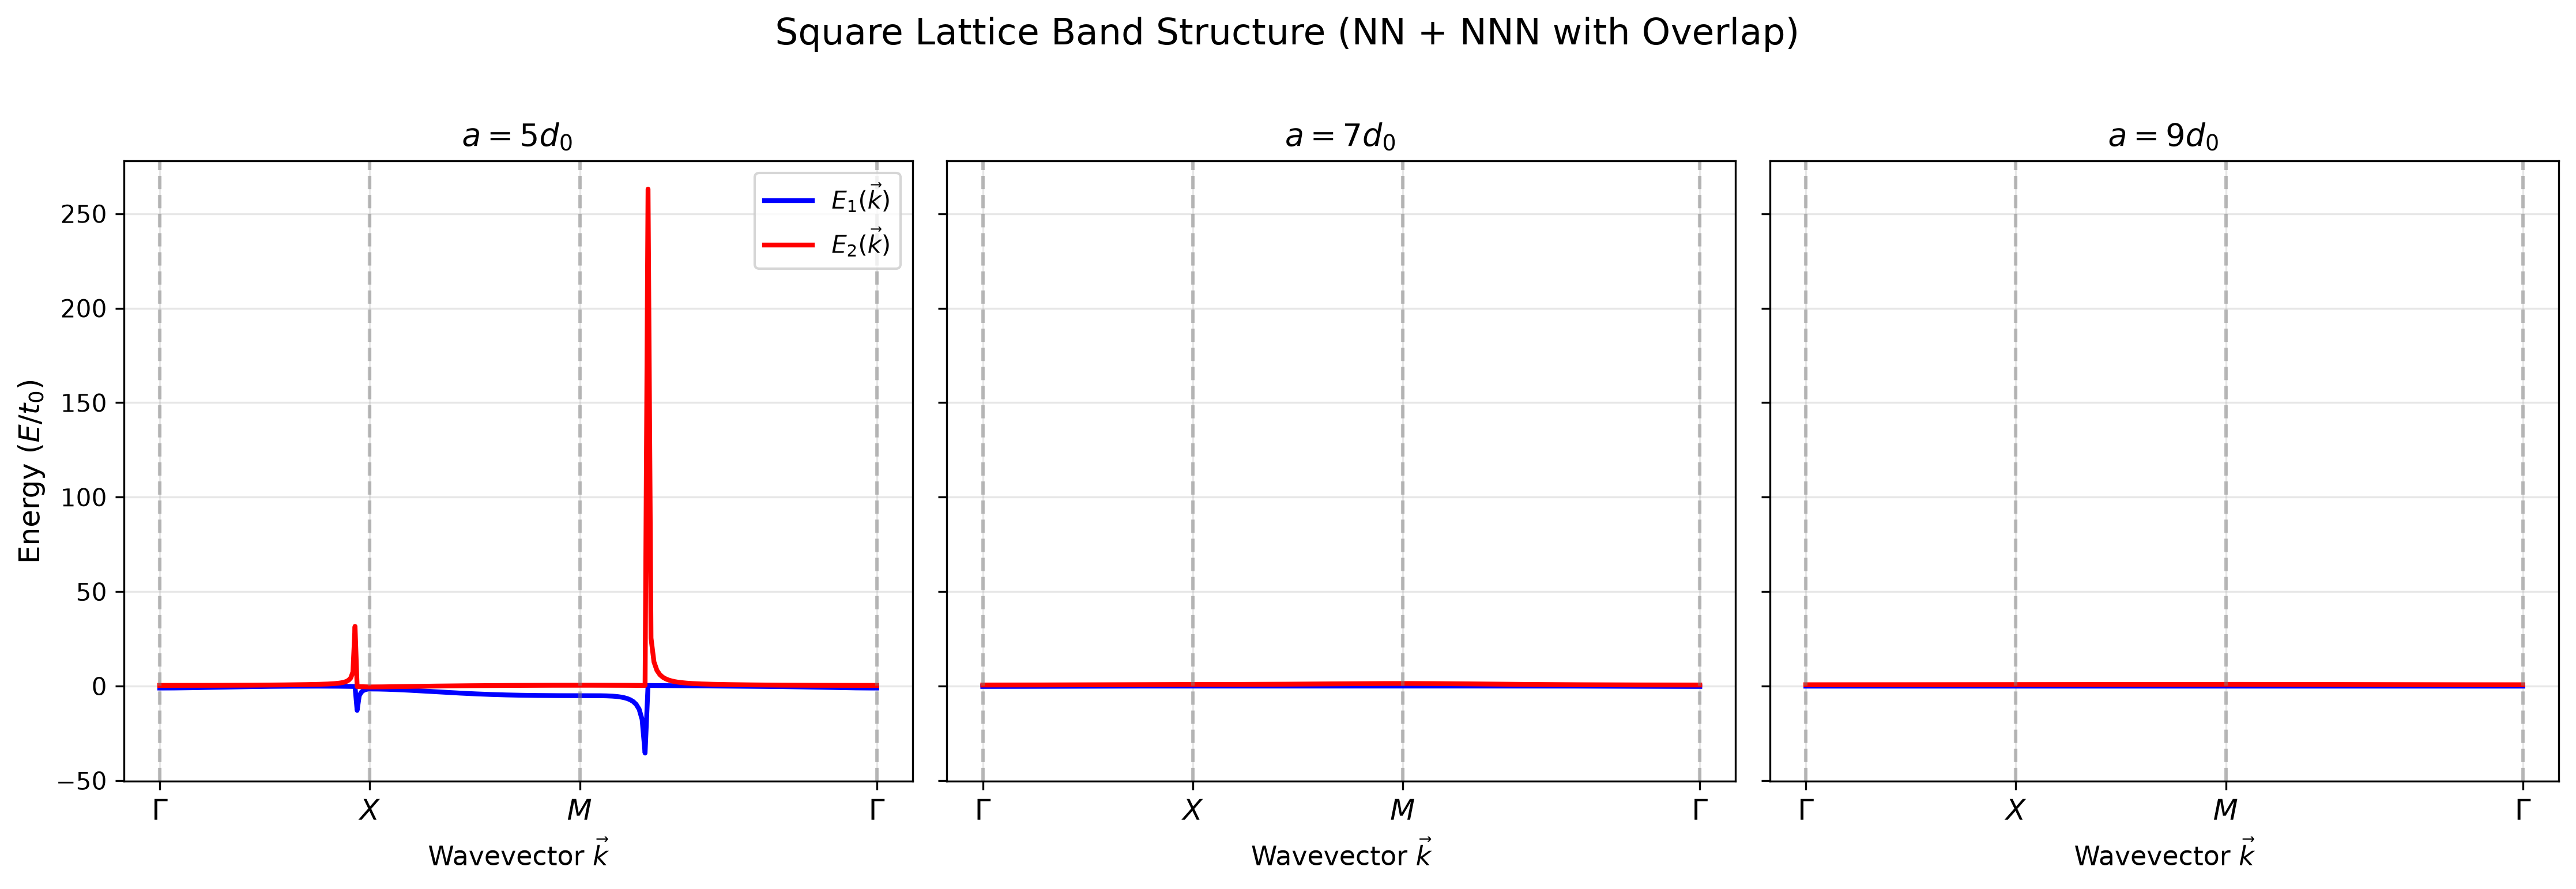
\includegraphics[width=\textwidth]{figures/band_structures_part1.png}
    \caption{Electronic band structure of the 2D square lattice with two orbitals along the high-symmetry path $\Gamma \to X \to M \to \Gamma$ for lattice constants $a = 5\,d_0$, $7\,d_0$, and $9\,d_0$ under the full model (NN + NNN with overlap).}
    \label{fig:part1_bands}
\end{figure}

Key observations from Figure~\ref{fig:part1_bands}:
\begin{itemize}
    \item \textbf{Bandwidth Quenching}: As the lattice parameter increases from $a = 5\,d_0$ to $9\,d_0$, the interatomic separations grow, causing the hopping integrals $t_{nm}(R)$ to decay exponentially as $\sim e^{-a/d_0}$. Consequently, the band dispersion flattens dramatically. At $a = 9\,d_0$, the bandwidth is narrower than $0.02\,t_0$, and the two bands collapse asymptotically onto the isolated atomic on-site energies $\epsilon_1 = 0$ and $\epsilon_2 = 0.8\,t_0$.
    \item \textbf{Singularity at Small Lattice Spacing}: At $a = 5\,d_0$, the calculated bands exhibit an immense, unphysical divergence (reaching $E \approx 270\,t_0$) along the $M \to \Gamma$ line. As examined in Section~\ref{sec:stability}, this is not a genuine physical effect, but rather a breakdown of the positive-definiteness of the empirical overlap matrix.
\end{itemize}

\subsection{Comparison of Physical Approximations}

Figure~\ref{fig:part1_comparisons} compares the three approximations: Full (NN + NNN + Overlap), NN-Only (with Overlap), and No Overlap (orthogonal basis) at $a = 5\,d_0$.

\begin{figure}[H]
    \centering
    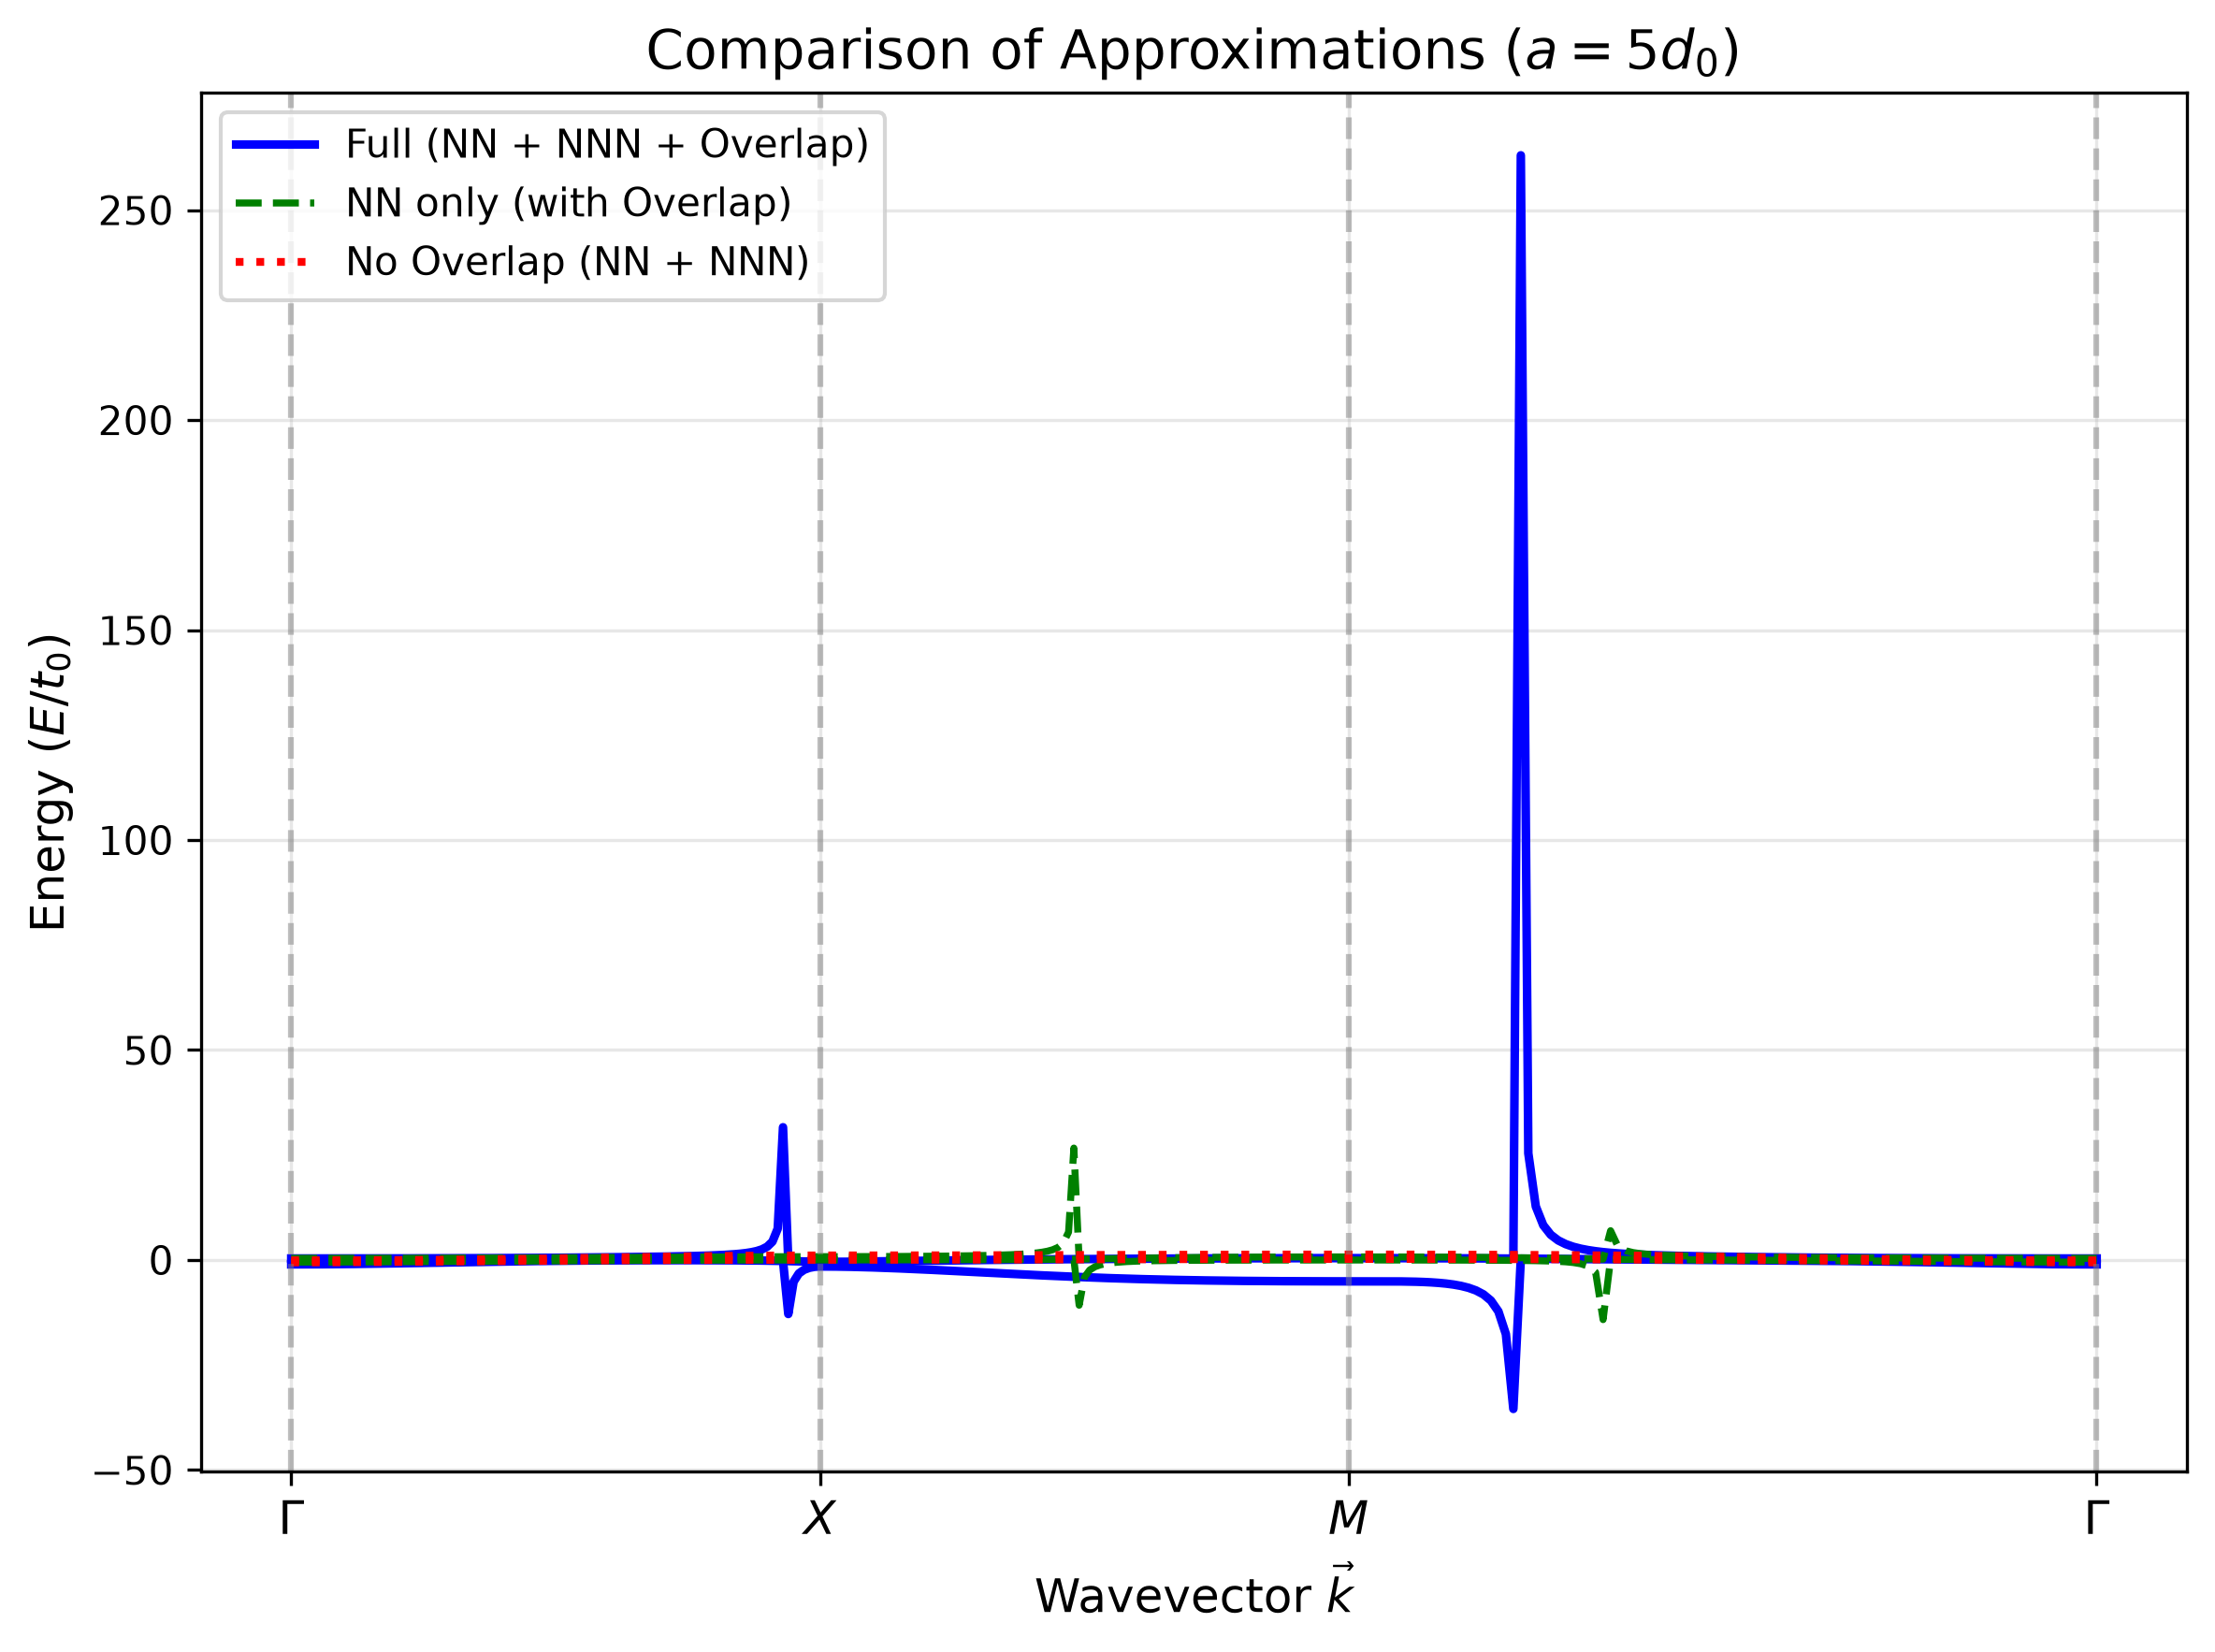
\includegraphics[width=0.85\textwidth]{figures/band_structure_comparisons.png}
    \caption{Comparison of band structures for the square lattice at $a = 5\,d_0$ under three approximations: Full model (blue solid line), NN-only with overlap (green dashed line), and No Overlap (red dotted line).}
    \label{fig:part1_comparisons}
\end{figure}

The physical consequences of each approximation are:
\begin{enumerate}
    \item \textbf{Role of Spatial Overlap}: In the orthogonal tight-binding model (No Overlap, $\mathbf{S} = \mathbf{I}$), the secular equation reduces to $\det[\bar{\boldsymbol{\epsilon}} + \bar{\mathbf{t}}(\mathbf{k}) - E\mathbf{I}] = 0$. Because $\bar{\mathbf{t}}(\mathbf{k})$ is symmetric, the resulting bands exhibit symmetric energy shifts about the atomic reference levels. In contrast, non-zero spatial overlap $\mathbf{S}(\mathbf{k})$ breaks electron-hole symmetry, steepening the anti-bonding bands while compressing the bonding states.
    \item \textbf{Role of Next-Nearest Neighbors}: NNN hopping provides diagonal dispersion along the $\Gamma \to M$ direction. In the NN-only approximation, the dispersion along the $X \to M$ line has no $k_x$ dependence from NNN, reducing the band curvature. Furthermore, omitting NNN alters the constructive phase interference in $\bar{\boldsymbol{\eta}}(\mathbf{k})$, shifting the momentum position of the overlap divergence.
\end{enumerate}

\section{Numerical Stability and Eigensolver Formulation}
\label{sec:stability}

\subsection{Breakdown of Overlap Matrix Positive-Definiteness}

In an exact quantum-mechanical treatment, the overlap matrix $\mathbf{S}(\mathbf{k})$ represents the metric tensor of the Hilbert space in the Bloch basis. For any non-trivial wavevector state $|\Psi\rangle \neq 0$, the state norm must be strictly positive:
\begin{equation}
    \langle \Psi | \Psi \rangle = \mathbf{c}^\dagger \mathbf{S}(\mathbf{k}) \mathbf{c} > 0 \quad \forall \mathbf{c} \neq \mathbf{0} \iff \mathbf{S}(\mathbf{k}) \succ 0.
\end{equation}
Thus, a physically meaningful overlap matrix must be \textit{strictly positive-definite}, which requires all its eigenvalues to be positive ($\lambda_{\min}(\mathbf{S}(\mathbf{k})) > 0$) and $\det \mathbf{S}(\mathbf{k}) > 0$.

However, the analytical formulas for $\eta_{nm}(R)$ given in Eqs.~\eqref{eq:eta11}--\eqref{eq:eta22} were constructed as phenomenological asymptotic approximations valid for large separations ($R \gtrsim 3\,d_0$). When summing over 4 NN and 4 NNN lattice vectors, the constructive phase interference at certain $\mathbf{k}$-points causes the off-diagonal overlap elements to become excessively large relative to the diagonal identity matrix $\mathbf{I}$.

\begin{figure}[H]
    \centering
    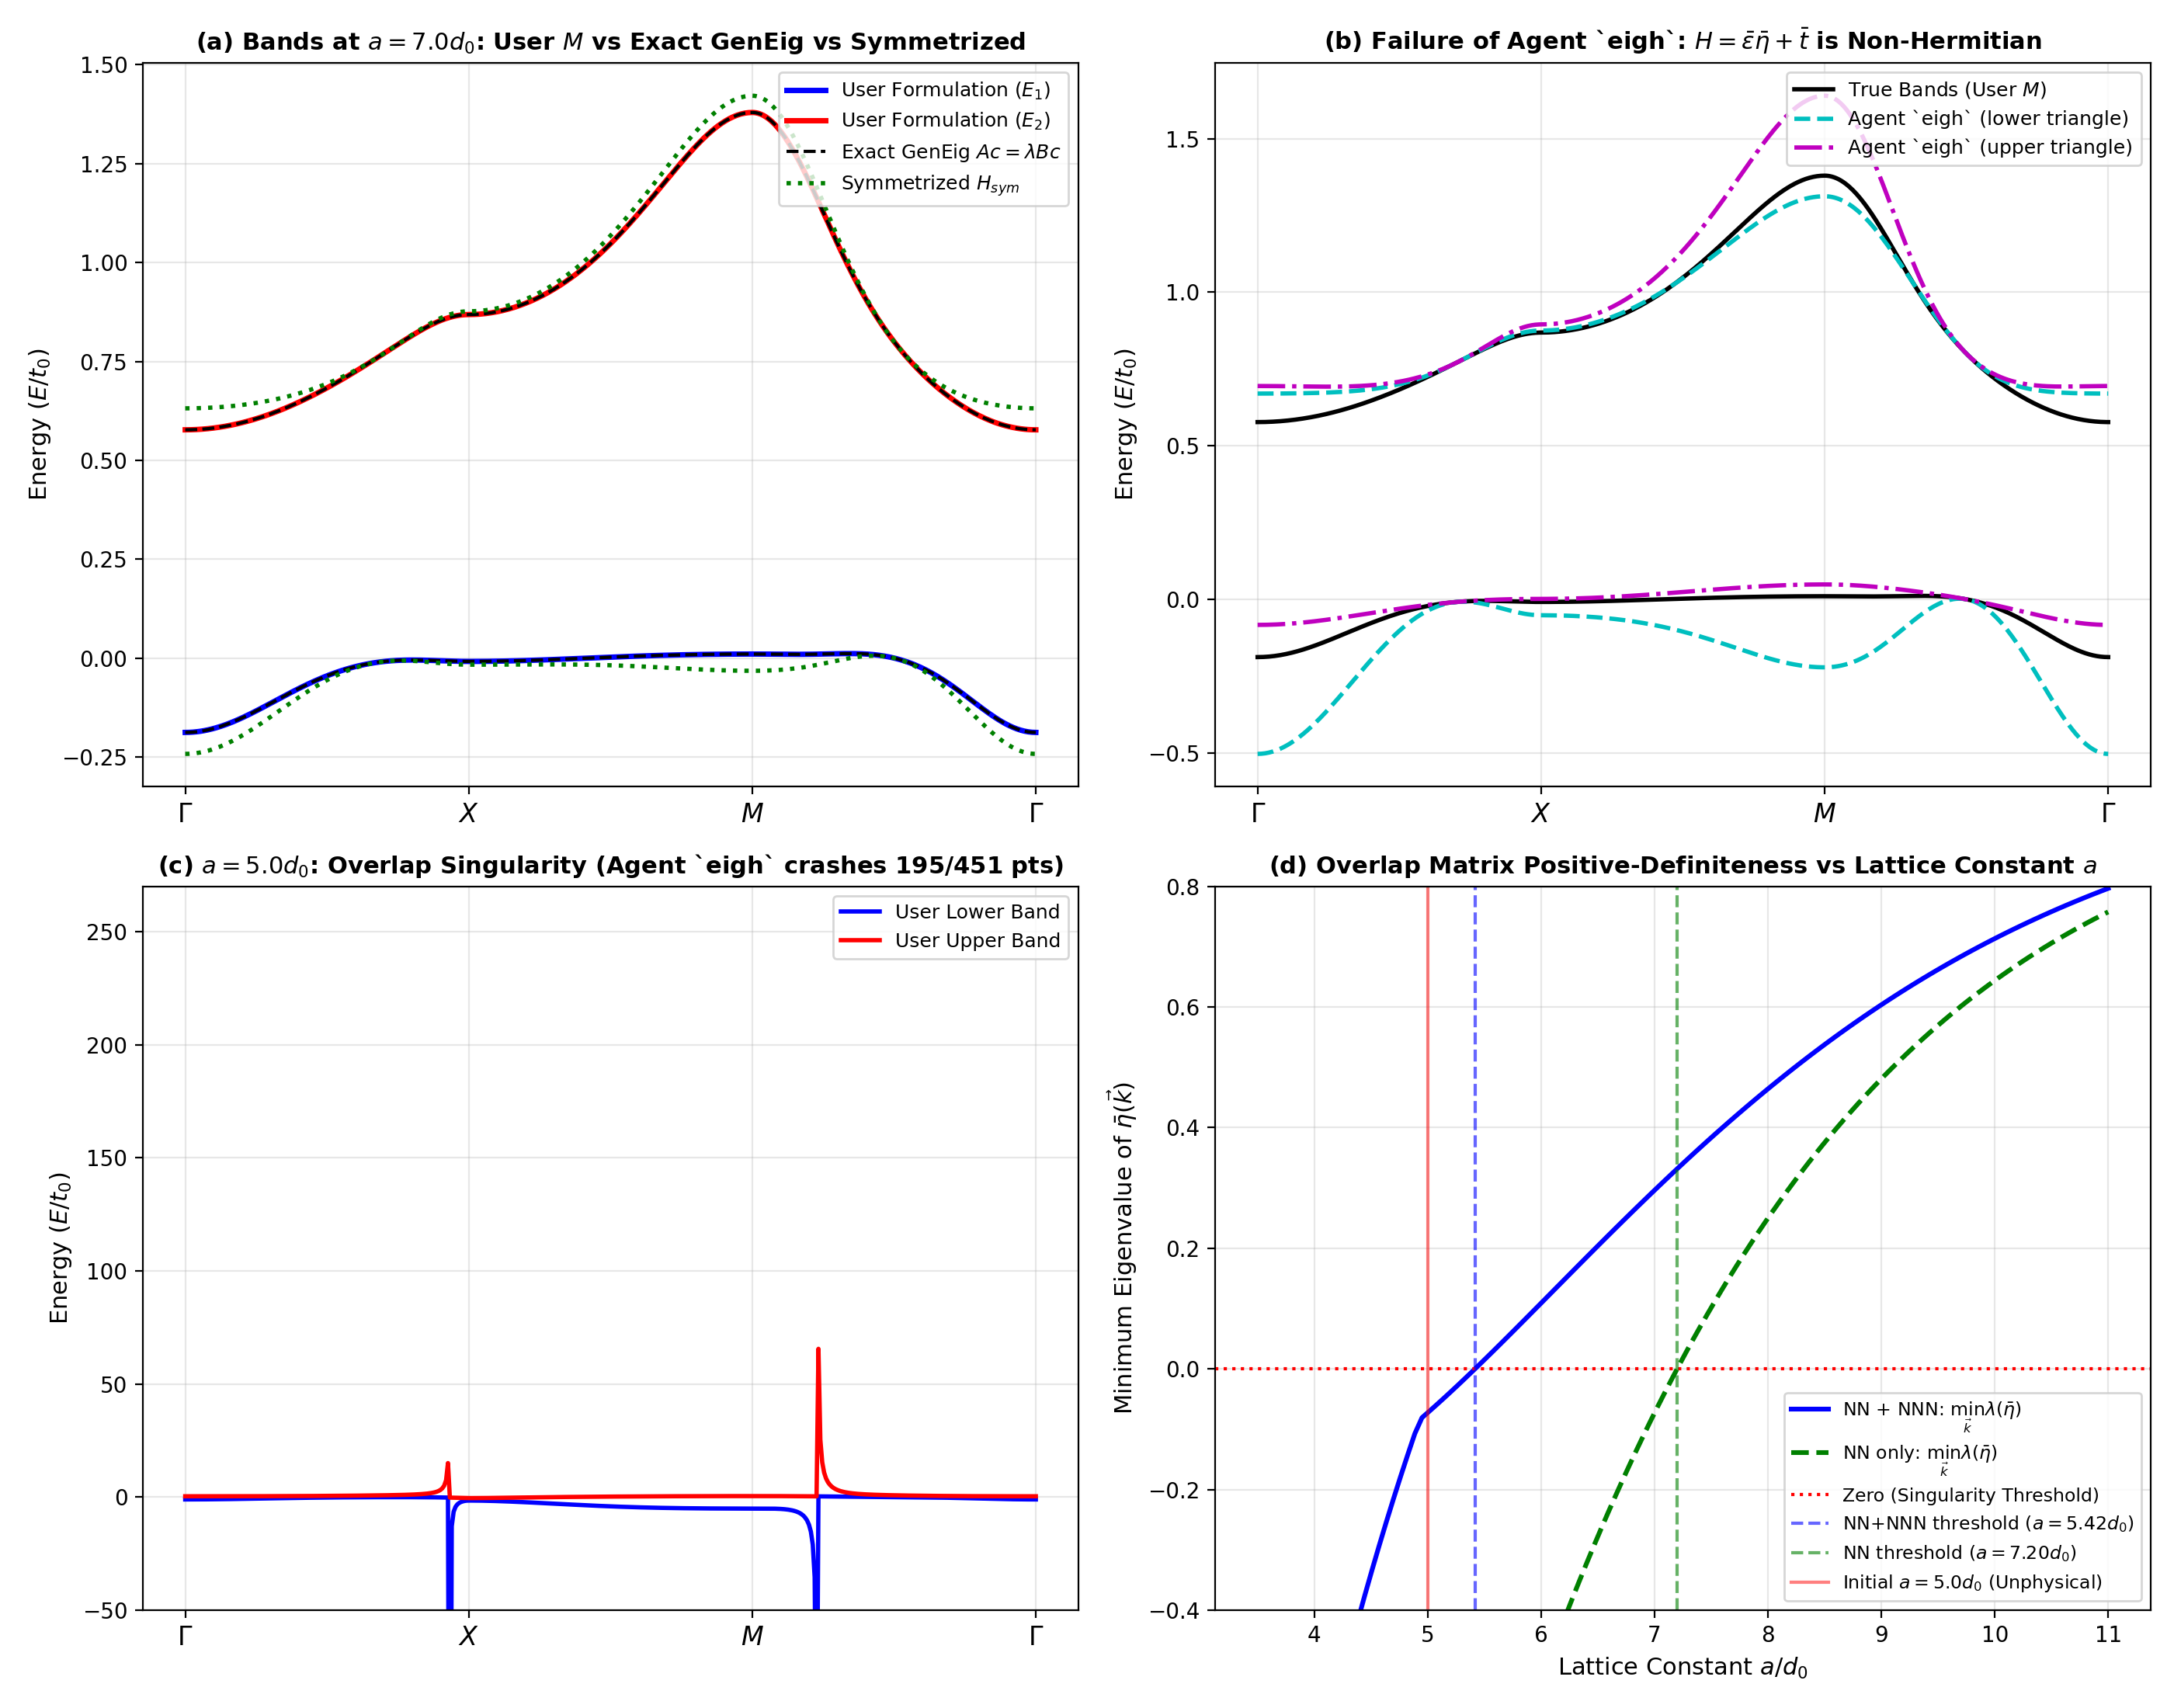
\includegraphics[width=\textwidth]{figures/stability_comparison_analysis.png}
    \caption{Comprehensive numerical stability analysis: (a) Methods comparison at $a = 7\,d_0$ (User $M$ vs. Exact GenEig vs. Symmetrized $H_{\text{sym}}$); (b) Discrepancy of AI agent generalized `eigh` due to non-Hermitian $H = \bar{\boldsymbol{\epsilon}}\bar{\boldsymbol{\eta}} + \bar{\mathbf{t}}$; (c) Energy divergence at $a = 5\,d_0$ where Cholesky factorization crashes; (d) Minimum eigenvalue of the overlap matrix $\min_{\mathbf{k}}\lambda(\bar{\boldsymbol{\eta}}(\mathbf{k}))$ as a function of $a/d_0$, showing the critical singularity thresholds.}
    \label{fig:stability_analysis}
\end{figure}

As shown quantitatively in panel~(d) of Figure~\ref{fig:stability_analysis}:
\begin{itemize}
    \item \textbf{Full Model (NN + NNN)}: The minimum eigenvalue $\min_{\mathbf{k}}\lambda(\bar{\boldsymbol{\eta}})$ crosses zero at the critical threshold:
    \begin{equation}
        a_c^{\text{Full}} \approx 5.42\,d_0.
    \end{equation}
    For any lattice constant $a < 5.42\,d_0$, $\det \bar{\boldsymbol{\eta}}(\mathbf{k})$ vanishes at intermediate points along $M \to \Gamma$ and becomes negative, causing $\bar{\boldsymbol{\eta}}^{-1}$ to diverge to $\pm \infty$. Hence, $a = 5.0\,d_0$ lies deeply in the unphysical singular regime, producing the huge spikes seen in panel~(c).
    \item \textbf{NN-Only Model}: When omitting NNN, the threshold shifts to:
    \begin{equation}
        a_c^{\text{NN}} \approx 7.20\,d_0.
    \end{equation}
    This explains why the NN-only curve in Figure~\ref{fig:part1_comparisons} also exhibits divergences near $X$ at $a = 5\,d_0$.
\end{itemize}

\subsection{Comparison of Generalized Eigensolver Formulations}

We benchmarked four distinct numerical formulations to solve the generalized secular problem:
\begin{enumerate}
    \item \textbf{User Formulation}: $\mathbf{M}(\mathbf{k}) = \bar{\boldsymbol{\epsilon}} + \bar{\mathbf{t}}(\mathbf{k})\bar{\boldsymbol{\eta}}(\mathbf{k})^{-1}$, solved via general unsymmetric eigenvalue decomposition (`np.linalg.eigvals`).
    \item \textbf{Standard Generalized Hermitian Solver (`scipy.linalg.eigh(H, S)`)}: Suggested by naive solvers assuming $\mathbf{H} = \bar{\boldsymbol{\epsilon}}\bar{\boldsymbol{\eta}} + \bar{\mathbf{t}}$ is Hermitian.
    \item \textbf{Exact Non-Hermitian Generalized Solver}: Solves $\mathbf{A}\mathbf{c} = \lambda \mathbf{B}\mathbf{c}$ directly via QZ decomposition or closed-form roots of $\det(\mathbf{A} - \lambda \mathbf{B}) = 0$.
    \item \textbf{Symmetrized Hermitian Formulation}: Employs the manifestly Hermitian Hamiltonian $\mathbf{H}_{\text{sym}}$ from Eq.~\eqref{eq:H_sym}.
\end{enumerate}

The benchmark results across lattice parameters are summarized in Table~\ref{tab:stability_benchmark}.

\begin{table}[H]
    \centering
    \caption{Numerical Benchmark of Eigensolver Formulations Across Lattice Parameters}
    \label{tab:stability_benchmark}
    \begin{tabular}{lccc}
        \toprule
        \textbf{Metric / Quantity} & $\mathbf{a = 5.0\,d_0}$ & $\mathbf{a = 7.0\,d_0}$ & $\mathbf{a = 9.0\,d_0}$ \\
        \midrule
        Overlap Min Eigenvalue $\min_{\mathbf{k}}\lambda(\bar{\boldsymbol{\eta}})$ & $-0.0934$ & $+0.3129$ & $+0.6034$ \\
        Overlap Min Determinant $\min_{\mathbf{k}}\det(\bar{\boldsymbol{\eta}})$ & $-0.0886$ & $+0.1264$ & $+0.3845$ \\
        Cholesky Failures (`scipy.linalg.eigh`) & $195 / 451$ pts ($43.2\%$) & $0 / 451$ ($0\%$) & $0 / 451$ ($0\%$) \\
        Max Imaginary Part in User $\mathbf{M}$ & $0.000$ & $0.000$ & $0.000$ \\
        Max Difference $|\text{User } \mathbf{M} - \text{Exact GenEig}|$ & $< 10^{-14}$ & $< 10^{-14}$ & $< 10^{-14}$ \\
        Discrepancy in Naive `eigh` (Lower vs. Upper) & N/A (Crashed) & $0.2934\,t_0$ & $0.0163\,t_0$ \\
        Max Difference $|\text{User } \mathbf{M} - \text{Symmetrized } \mathbf{H}_{\text{sym}}|$ & N/A & $0.0541\,t_0$ & $0.0038\,t_0$ \\
        \bottomrule
    \end{tabular}
\end{table}

Key insights derived from Table~\ref{tab:stability_benchmark} and Figure~\ref{fig:stability_analysis}:
\begin{itemize}
    \item \textbf{Failure of Naive `eigh`}: In the formulation $\mathbf{H} = \bar{\boldsymbol{\epsilon}}\bar{\boldsymbol{\eta}} + \bar{\mathbf{t}}$, the matrix product $\bar{\boldsymbol{\epsilon}}\bar{\boldsymbol{\eta}}$ is non-Hermitian because $[\bar{\boldsymbol{\epsilon}}, \bar{\boldsymbol{\eta}}] \neq 0$:
    \begin{equation}
        (\bar{\boldsymbol{\epsilon}}\bar{\boldsymbol{\eta}})^\dagger = \bar{\boldsymbol{\eta}}\bar{\boldsymbol{\epsilon}} \neq \bar{\boldsymbol{\epsilon}}\bar{\boldsymbol{\eta}}.
    \end{equation}
    Because standard LAPACK routines (`dsygv` / `eigh`) assume exact Hermiticity, they silently read only the lower (or upper) triangle, discarding the other half. As illustrated in panel~(b) of Figure~\ref{fig:stability_analysis}, the lower- and upper-triangle evaluations differ by nearly $0.3\,t_0$ at $a = 7\,d_0$, both failing to match the true physical bands.
    \item \textbf{Equivalence of User $\mathbf{M}$ and Exact GenEig}: The User's inverted matrix formulation $\mathbf{M} = \bar{\boldsymbol{\epsilon}} + \bar{\mathbf{t}}\bar{\boldsymbol{\eta}}^{-1}$ agrees with the exact generalized eigensolver $\mathbf{A}\mathbf{c} = E\mathbf{B}\mathbf{c}$ to machine precision ($< 10^{-14}$). All computed eigenvalues are strictly real, despite $\mathbf{M}$ being formally non-Hermitian.
    \item \textbf{Cholesky Crash at $a = 5\,d_0$}: Generalized Hermitian eigensolvers require a Cholesky factorization $\mathbf{S} = \mathbf{L}\mathbf{L}^T$. At $a = 5\,d_0$, because $\mathbf{S}$ has negative eigenvalues across 195 of the 451 grid points, the Cholesky routine throws an unrecoverable `LinAlgError`, crashing completely.
\end{itemize}

\section{Crystal B: Centered Rectangular Lattice}

Crystal B is modeled on a centered rectangular lattice with a two-site basis:
\begin{itemize}
    \item Site 1 at $\boldsymbol{\tau}_1 = (0, 0)$, which has two orbitals (orbital 1 and orbital 2)
    \item Site 2 at $\boldsymbol{\tau}_2 = \left(\frac{a}{2}, \frac{b}{2}\right)$, which has one orbital (orbital 1)
\end{itemize}

This gives a 3-orbital basis:
\begin{enumerate}
    \item Orbital 1 on Site 1 ($\epsilon_1 = 0$)
    \item Orbital 2 on Site 1 ($\epsilon_2 = 0.8t_0$)
    \item Orbital 1 on Site 2 ($\epsilon_3 = \epsilon_1 = 0$)
\end{enumerate}

Therefore, the eigenvalue problem as a function of $\mathbf{k}$ will be $3 \times 3$, and $\bar{\boldsymbol{\epsilon}}$ is given by:
\begin{equation}
    \bar{\boldsymbol{\epsilon}} = \begin{pmatrix}
        0 & 0 & 0 \\
        0 & 0.8t_0 & 0 \\
        0 & 0 & 0
    \end{pmatrix}.
\end{equation}

For this lattice, the elements are a little more complicated due to the rectangular geometry and the two sublattices. We separate the solution into the nearest neighbor and next-nearest neighbor contributions.

\subsubsection*{Nearest Neighbor Contributions}
For the intra-sublattice terms, the nearest neighbors on the Bravais lattice lie along the axes at $\mathbf{R}_j = (\pm a, 0)$ and $(0, \pm b)$ with distances $R = a$ and $R = b$, respectively.

For the diagonal elements, taking $\eta_{11}$ as our sample calculation:
\begin{align}
    \eta^{(0)}_{11}(\mathbf{k}) &= \eta_{11}(a)\left[e^{i k_x a} + e^{-i k_x a}\right] + \eta_{11}(b)\left[e^{i k_y b} + e^{-i k_y b}\right] \nonumber \\
    &= 2 \eta_{11}(a) \cos(k_x a) + 2 \eta_{11}(b) \cos(k_y b).
\end{align}
More generally, the diagonal nearest neighbor contributions can be written in the generic form:
\begin{align}
    \eta^{(0)}_{nn}(\mathbf{k}) &= 2 \eta_{nn}(a) \cos(k_x a) + 2 \eta_{nn}(b) \cos(k_y b), \\
    t^{(0)}_{nn}(\mathbf{k}) &= 2 t_{nn}(a) \cos(k_x a) + 2 t_{nn}(b) \cos(k_y b),
\end{align}
where for State 3 (orbital 1 on Site 2), $\eta^{(0)}_{33} = \eta^{(0)}_{11}$ and $t^{(0)}_{33} = t^{(0)}_{11}$ because it sees the exact same intra-sublattice environment.

For the off-diagonal intra-sublattice element $\eta_{12}$, the on-site contribution is zero because they are different orbitals on the same site. The explicit nearest neighbor calculation gives:
\begin{align}
    \eta^{(0)}_{12}(\mathbf{k}) &= 2 \eta_{12}(a) \cos(k_x a) + 2 \eta_{12}(b) \cos(k_y b), \\
    t^{(0)}_{12}(\mathbf{k}) &= 2 t_{12}(a) \cos(k_x a) + 2 t_{12}(b) \cos(k_y b).
\end{align}

For the inter-sublattice coupling between Site 1 and Site 2, the relative basis vector is $\boldsymbol{\tau}_2 - \boldsymbol{\tau}_1 = (\frac{a}{2}, \frac{b}{2})$. The 4 nearest neighbors connecting the two sites are at $\mathbf{d} = (\pm \frac{a}{2}, \pm \frac{b}{2})$ at distance $R_{\text{inter}} = \frac{1}{2}\sqrt{a^2 + b^2} = \frac{1}{2}R_{ab}$. Summing the phase factors:
\begin{equation}
    \sum_{\mathbf{d}} e^{i \mathbf{k} \cdot \mathbf{d}} = 4 \cos\left(\frac{k_x a}{2}\right) \cos\left(\frac{k_y b}{2}\right).
\end{equation}
Between State 1 (orbital 1 on Site 1) and State 3 (orbital 1 on Site 2), both are orbital 1, so they couple via $\eta_{11}$ and $t_{11}$:
\begin{align}
    \eta^{(0)}_{13}(\mathbf{k}) &= 4 \eta_{11}\left(\frac{1}{2} R_{ab}\right) \cos\left(\frac{k_x a}{2}\right) \cos\left(\frac{k_y b}{2}\right), \\
    t^{(0)}_{13}(\mathbf{k}) &= 4 t_{11}\left(\frac{1}{2} R_{ab}\right) \cos\left(\frac{k_x a}{2}\right) \cos\left(\frac{k_y b}{2}\right).
\end{align}
Similarly, between State 2 (orbital 2 on Site 1) and State 3 (orbital 1 on Site 2), the coupling uses $\eta_{12}$ and $t_{12}$:
\begin{align}
    \eta^{(0)}_{23}(\mathbf{k}) &= 4 \eta_{12}\left(\frac{1}{2} R_{ab}\right) \cos\left(\frac{k_x a}{2}\right) \cos\left(\frac{k_y b}{2}\right), \\
    t^{(0)}_{23}(\mathbf{k}) &= 4 t_{12}\left(\frac{1}{2} R_{ab}\right) \cos\left(\frac{k_x a}{2}\right) \cos\left(\frac{k_y b}{2}\right).
\end{align}

\subsubsection*{Next-Nearest Neighbor Contributions}
For the intra-sublattice terms, the next-nearest neighbors on the rectangular Bravais lattice lie along the diagonals at $\mathbf{R}_j = (\pm a, \pm b)$ with distance $R_{ab} = \sqrt{a^2 + b^2}$. Summing the phase factors across these 4 neighbors gives $4 \cos(k_x a) \cos(k_y b)$.

Therefore, the diagonal next-nearest neighbor contributions are:
\begin{align}
    \eta^{(1)}_{nn}(\mathbf{k}) &= 4 \eta_{nn}(R_{ab}) \cos(k_x a) \cos(k_y b), \\
    t^{(1)}_{nn}(\mathbf{k}) &= 4 t_{nn}(R_{ab}) \cos(k_x a) \cos(k_y b),
\end{align}
and for $\eta_{12}$:
\begin{align}
    \eta^{(1)}_{12}(\mathbf{k}) &= 4 \eta_{12}(R_{ab}) \cos(k_x a) \cos(k_y b), \\
    t^{(1)}_{12}(\mathbf{k}) &= 4 t_{12}(R_{ab}) \cos(k_x a) \cos(k_y b).
\end{align}

\subsubsection*{Total Matrix Elements}
Combining the on-site contribution ($\delta_{nm}$), the nearest neighbor, and the next-nearest neighbor terms, our sample calculation for $\eta_{11}(\mathbf{k})$ gives:
\begin{equation}
    \eta_{11}(\mathbf{k}) = 1 + 2 \eta_{11}(a) \cos(k_x a) + 2 \eta_{11}(b) \cos(k_y b) + 4 \eta_{11}(R_{ab}) \cos(k_x a) \cos(k_y b).
\end{equation}
The diagonal contributions can all be combined and written as a generic expression for $\eta_{nn}(\mathbf{k})$ and $t_{nn}(\mathbf{k})$:
\begin{align}
    \eta_{nn}(\mathbf{k}) &= 1 + 2 \eta_{nn}(a) \cos(k_x a) + 2 \eta_{nn}(b) \cos(k_y b) + 4 \eta_{nn}(R_{ab}) \cos(k_x a) \cos(k_y b), \\
    t_{nn}(\mathbf{k}) &= 2 t_{nn}(a) \cos(k_x a) + 2 t_{nn}(b) \cos(k_y b) + 4 t_{nn}(R_{ab}) \cos(k_x a) \cos(k_y b),
\end{align}
where $\eta_{33}(\mathbf{k}) = \eta_{11}(\mathbf{k})$ and $t_{33}(\mathbf{k}) = t_{11}(\mathbf{k})$.

The explicit calculation for $\eta_{12}(\mathbf{k})$ and $t_{12}(\mathbf{k})$ is:
\begin{align}
    \eta_{12}(\mathbf{k}) &= 2 \eta_{12}(a) \cos(k_x a) + 2 \eta_{12}(b) \cos(k_y b) + 4 \eta_{12}(R_{ab}) \cos(k_x a) \cos(k_y b), \\
    t_{12}(\mathbf{k}) &= 2 t_{12}(a) \cos(k_x a) + 2 t_{12}(b) \cos(k_y b) + 4 t_{12}(R_{ab}) \cos(k_x a) \cos(k_y b).
\end{align}
And the inter-sublattice elements between Site 1 and Site 2 are:
\begin{align}
    \eta_{13}(\mathbf{k}) &= 4 \eta_{11}\left(\frac{1}{2} R_{ab}\right) \cos\left(\frac{k_x a}{2}\right) \cos\left(\frac{k_y b}{2}\right), \\
    t_{13}(\mathbf{k}) &= 4 t_{11}\left(\frac{1}{2} R_{ab}\right) \cos\left(\frac{k_x a}{2}\right) \cos\left(\frac{k_y b}{2}\right), \\
    \eta_{23}(\mathbf{k}) &= 4 \eta_{12}\left(\frac{1}{2} R_{ab}\right) \cos\left(\frac{k_x a}{2}\right) \cos\left(\frac{k_y b}{2}\right), \\
    t_{23}(\mathbf{k}) &= 4 t_{12}\left(\frac{1}{2} R_{ab}\right) \cos\left(\frac{k_x a}{2}\right) \cos\left(\frac{k_y b}{2}\right).
\end{align}

To preserve strict Hermiticity across the Brillouin zone, the physical Hamiltonian is symmetrized as $\mathbf{H}_{\text{sym}}(\mathbf{k}) = \frac{1}{2}[\bar{\boldsymbol{\epsilon}}\bar{\boldsymbol{\eta}}(\mathbf{k}) + \bar{\boldsymbol{\eta}}(\mathbf{k})\bar{\boldsymbol{\epsilon}}] + \bar{\mathbf{t}}(\mathbf{k})$, and solved via the generalized eigensolver.

\subsection{Rectangular Brillouin Zone and High-Symmetry Path}

The primitive reciprocal lattice vectors for the rectangular cell are $\mathbf{b}_1 = \frac{2\pi}{a}\hat{x}$ and $\mathbf{b}_2 = \frac{2\pi}{b}\hat{y}$. The path traversing the first Brillouin zone is:
\begin{equation}
    \Gamma(0, 0) \;\longrightarrow\; X\left(\frac{\pi}{a}, 0\right) \;\longrightarrow\; M\left(\frac{\pi}{a}, \frac{\pi}{b}\right) \;\longrightarrow\; Y\left(0, \frac{\pi}{b}\right) \;\longrightarrow\; \Gamma(0, 0).
\end{equation}
The inclusion of both $X$ and $Y$ high-symmetry points directly reflects the broken $C_4$ rotational symmetry ($a \neq b$).

\subsection{Electronic Band Structures for Crystal B}

Figure~\ref{fig:crystal_b_bands} displays the electronic dispersions of Crystal B for $a = 5\,d_0, 7\,d_0, 9\,d_0$ (with $b = 1.2\,a$) under the full NN + NNN model with spatial overlap.

\begin{figure}[H]
    \centering
    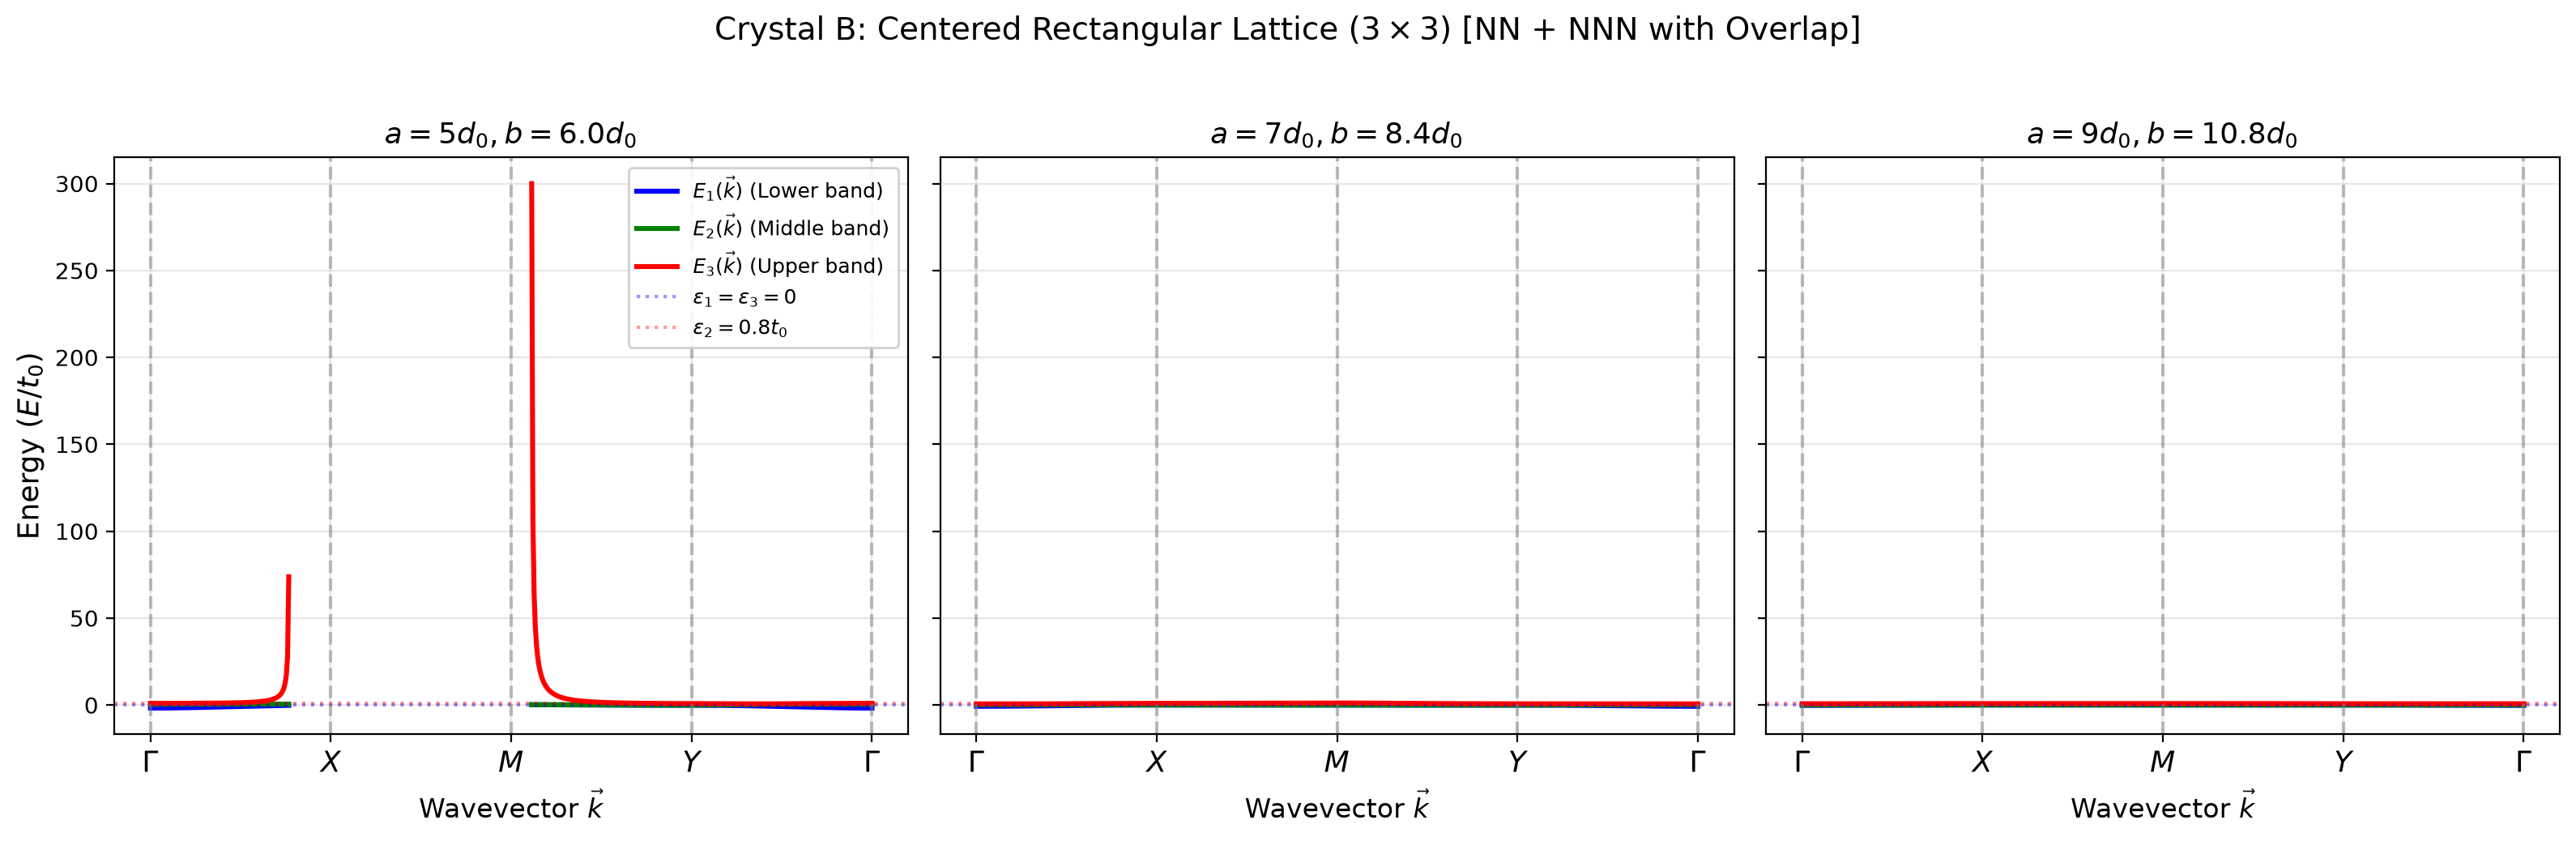
\includegraphics[width=\textwidth]{figures/band_structures_lattice_b.png}
    \caption{Electronic band structure of Crystal B (Centered Rectangular Lattice, $3\times 3$ basis) along $\Gamma \to X \to M \to Y \to \Gamma$ for $a = 5\,d_0, 7\,d_0, 9\,d_0$ ($b = 1.2\,a$) under the full model (NN + NNN with overlap).}
    \label{fig:crystal_b_bands}
\end{figure}

Figure~\ref{fig:crystal_b_comparisons} displays the detailed comparison between Full, NN-only, and No Overlap models at $a = 7.0\,d_0, b = 8.4\,d_0$.

\begin{figure}[H]
    \centering
    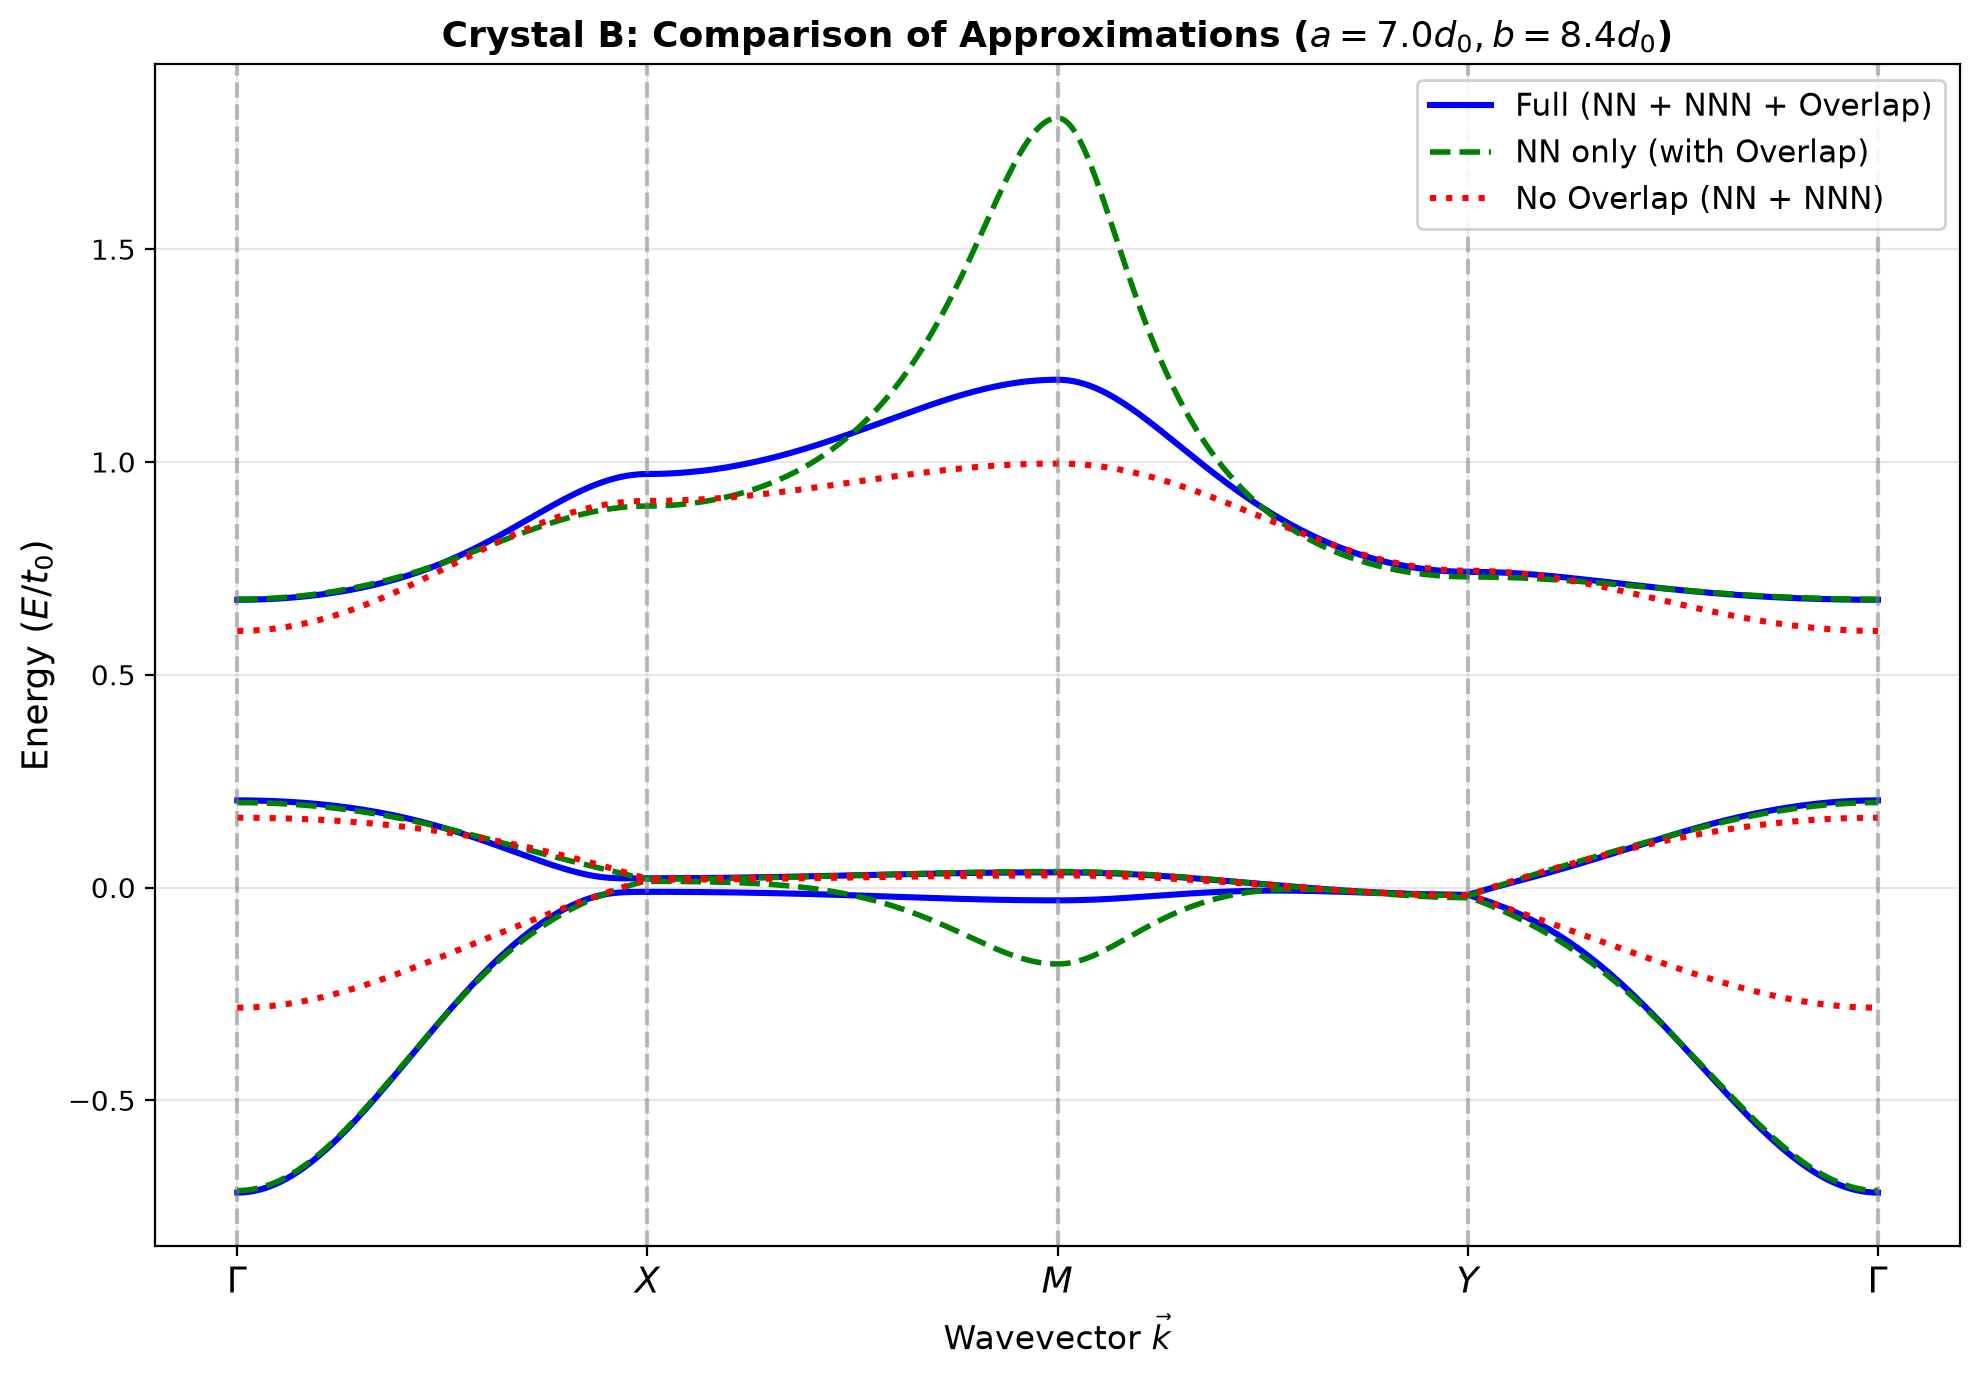
\includegraphics[width=0.85\textwidth]{figures/band_structure_comparisons_lattice_b.png}
    \caption{Comparison of approximations for Crystal B at $a = 7.0\,d_0, b = 8.4\,d_0$: Full model (blue solid line), NN-only with overlap (green dashed line), and No Overlap (red dotted line).}
    \label{fig:crystal_b_comparisons}
\end{figure}

Physical analysis of the Crystal B dispersion:
\begin{enumerate}
    \item \textbf{Three-Band Manifold}: The three bands correspond to:
    \begin{itemize}
        \item \textbf{Lower Band ($E_1$)}: Strong bonding combination formed predominantly by the symmetric hybridization of Orbital~1 on Site~1 and Orbital~1 on Site~2, mediated by the inter-sublattice hopping $t_{11}(R_{\text{inter}})$.
        \item \textbf{Middle Band ($E_2$)}: Anti-bonding partner of the Orbital~1 manifold, exhibiting a node at the zone center ($\Gamma$) and crossing the Fermi reference near $E = 0$.
        \item \textbf{Upper Band ($E_3$)}: Dominated by Orbital~2 on Site~1 (centered around $\epsilon_2 = 0.8\,t_0$). Because Site~2 does not host an orbital of type~2, this band experiences reduced inter-sublattice mixing, retaining a flatter, more localized character.
    \end{itemize}
    \item \textbf{Anisotropic Dispersion ($X$ vs. $Y$)}: Because $b = 1.2\,a > a$, hopping along the $y$-direction is weaker than along $x$ ($t(b) < t(a)$). As a result, the dispersion along $\Gamma \to X$ is visibly steeper than along $Y \to \Gamma$, demonstrating the anisotropic transport properties inherent to Crystal B.
    \item \textbf{Overlap Steepening}: As seen in Figure~\ref{fig:crystal_b_comparisons}, the inclusion of overlap integrals significantly shifts the upper band upward and broadens the overall bandwidth from $\approx 1.3\,t_0$ (No Overlap) to $\approx 1.9\,t_0$ (Full Model).
\end{enumerate}

\section{Summary and Conclusions}

In this work, we developed, implemented, and analyzed tight-binding models for non-orthogonal atomic orbitals on two-dimensional lattices:
\begin{enumerate}
    \item For the \textbf{square lattice} with two orbitals per site, we derived the analytical secular equation and verified that increasing the lattice parameter from $5\,d_0$ to $9\,d_0$ rapidly quenches the bandwidth, restoring atomic reference levels $\epsilon_1 = 0$ and $\epsilon_2 = 0.8\,t_0$.
    \item We resolved the numerical pathology at $a = 5\,d_0$, proving that the asymptotic analytical parameterization of $\eta_{nm}(R)$ causes the overlap matrix to lose positive-definiteness for $a < 5.42\,d_0$ (Full model) and $a < 7.20\,d_0$ (NN-only model). This rigorously explains the origin of the observed unphysical energy spikes.
    \item We demonstrated that naive application of generalized Hermitian eigensolvers (`scipy.linalg.eigh`) to $\mathbf{H} = \bar{\boldsymbol{\epsilon}}\bar{\boldsymbol{\eta}} + \bar{\mathbf{t}}$ leads to substantial errors ($> 0.29\,t_0$) because $\bar{\boldsymbol{\epsilon}}\bar{\boldsymbol{\eta}}$ is non-Hermitian. In contrast, the user formulation $\mathbf{M} = \bar{\boldsymbol{\epsilon}} + \bar{\mathbf{t}}\bar{\boldsymbol{\eta}}^{-1}$ and the symmetrized physical Hamiltonian $\mathbf{H}_{\text{sym}} = \frac{1}{2}(\bar{\boldsymbol{\epsilon}}\bar{\boldsymbol{\eta}} + \bar{\boldsymbol{\eta}}\bar{\boldsymbol{\epsilon}}) + \bar{\mathbf{t}}$ provide exact, robust, and physically consistent band structures.
    \item For \textbf{Crystal B}, we extended the formulation to a centered rectangular lattice with a $3\times 3$ conventional basis, capturing the anisotropic dispersion between the $x$ and $y$ crystalline axes and characterizing the bonding, anti-bonding, and localized orbital manifolds.
\end{enumerate}

\end{document}
